As discussed in \autoref{sec:intro}, randomness extraction is an efficient procedure for taking a sample from an imperfect random source, $X$ with distribution $p_X$, and "extracting" the \textit{pure}-randomness, i.e. being closer to uniformly distributed. A randomness extractor is a function that is applied to the output of a weakly random entropy source along with a short, uniformly random seed as input, and generates a highly random output that appears close to uniformly distributed and independent from the source \cite{vadhan2012}. Before formally defining a randomness extractor, we will define entropy, or how we measure the amount of randomness contained in a weak random source, as well as the statistical distance, or how we measure the closeness of the output distribution to the uniform distribution.

\begin{definition}\normalfont{\textbf{(Entropy)}}\label{def:entropy}
    The Shannon Entropy of a discrete random variable $X$ is defined as\[
        H(X) = \E\left[\log \frac{1}{p_i}\right] = \sum_{i \in X}p_i \log \frac{1}{p_i},
    \] where $p_i = \Pr[X=i]$.
\end{definition}

\begin{definition}\normalfont{\textbf{(Min- Entropy)}}\label{def:min_entropy}
    The min-entropy of a discrete random variable X is
    \[
        H_{\min}(X) = \min_{i} \log \frac{1}{p_i},
    \] or $H_{\min}(X)$ is the largest value of $k$ such that all outcomes have the probability of at most $2^{-k}$. 
    
In general, we like to guess the most likely outcome, and the probability that we are correct is $P_{\text{guess}}(X) = \max_x p_X(x)$. This results in an operational interpretation of the min-entropy as 
    \[
        H_{\min}(X) = -\log P_{\text{guess}}(X).
    \]
\end{definition}

When considering the above definitions, the question arises of why we use the min-entropy as the measure of uncertainty in cryptography as opposed to the Shannon entropy, which is used in information theory. Following Shannon’s approach, $i(x) =  -\log p_X(x)$ is the information gained when we observe $X$. Thus the Shannon entropy measured the average information gained, i.e.,  $H(X) = \sum_x p_X(x) i(x)$. However, when studying cryptography, we are interested in the worst case, not the average case, and the min-entropy $H_{\min}(X) = \min _x i(x)$ is precisely the smallest information gained. \autoref{fig:min_entropy} shows the difference between these quantities for a binary random variable. In general, $0\leq H_{\min}(X) \leq H(X)$.
\begin{figure}[!htb]
    \centering
    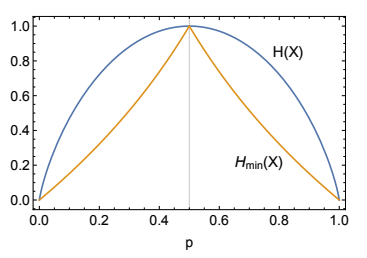
\includegraphics[scale=0.6]{Images/entropy.png}
    \caption{The comparison between Shannon entropy $H(X)$ and $\min$-entropy $H_{\min}(X)$ for a binary random variable $X = \set{0,1}$.}
    \label{fig:min_entropy}
\end{figure}

\begin{definition}\normalfont{\textbf{(Conditional Min-Entropy)}}
Consider two dependent random variables $X$ and $E$. The conditional min-entropy $H_{\min}(X|E)$ can be written as
\[H_{\min}(X|E) = -\log P_{\text{guess}}(X|E),\]
where $P_{\text{guess}}(X|E) = \max_x p_{X|E}(x|E)$.
\end{definition}

\begin{definition}\normalfont{\textbf{(Statistical Distance)}}
    Let $X$ and $Y$ be two random variables with range $\Ii$. Then the statistical distance between $X$ and $Y$ is defined as
    \[
        \Delta(X, Y) \equiv \frac{1}{2} \sum_{i \in \Ii} \left|\Pr[X=i]-\Pr[Y=i]\right|.
    \]
    For $\varepsilon \geq 0$, we define the notion of two distributions being $\varepsilon$-close as
    \[
        X \approx_{\varepsilon} Y \iff \Delta(X, Y) \leq \varepsilon.
    \]
\end{definition}

We now formally illustrate the process of randomness extraction. Consider a single party, Alice, who has access to an $n$-bit string, $x^n$, obtained from a source $X$ with distribution $p_{X}$. Perhaps, source $X$ is correlated to an additional
system or environment $E$. For example, $E$ could contain information about the generation of the source $X$ or an adversary who has gathered some prior information from protocols that include $X$. Alice has no access to system $E$ except the lower bound on the min-entropy of the source $X$ given environment $E$, i.e., $H_{\min}(X|E) \geq k$. In the task of randomness extraction, Alice’s goal is to construct \textit{randomness extractor}, denoted as $\ibeext$, that produces a
$m$-bit string $z^m$, which is close to the uniform distribution in the statistical distance and uncorrelated with environment $E$.

Before formally discussing the construction of a randomness extractor, consider an example that shows how to extract uniform bits from an i.i.d. (\textit{independent and identically distributed}) source.

\begin{example}Consider an i.i.d. binary source $X$ such that $X_i = 0$ w.p $p_0 = 1/4$ and $X_i = 1$ w.p $p_0 = 3/4$. Define the output $Z$ of the randomness extractor $Z = \ibeext(X) := X_1\oplus X_2\oplus \cdots \oplus X_n \in \set{0,1}$, i.e., the parity of all $n$-bits sequence of $X$. To find if we can extract uniformly random bits from an i.i.d. source, we need to show that $\Pr(Z=0) \approx 1/2 \pm \varepsilon$ for sufficiently small $\varepsilon > 0$, i.e., $Z \approx_{\varepsilon} \text{uniform}(\set{0,1})$.

Let's first examine how efficiently our strategy works for $n=2$. We need to compute
    $\Pr(Z=0) = \Pr(X_1 = 0, X_2 = 0) + \Pr(X_1 = 1, X_2 = 1) = p_0^2+p_1^2 = 0.625$. Similarly, we can compute $\Pr(Z=1) = 0.375$. Also, observe that $\Delta(X,U_2) = 0.25$ and $\Delta(Z,U_2) = 0.125$, where $U_2 \sim \text{uniform}(\set{0,1})$. In other words, the output distribution is not quite uniform, however, $Z$ is more closer to uniform distribution than $X$. Hence, following the above analysis for sufficiently large $n$, we observe that $Z \approx_\varepsilon U_2$.

\end{example}

In the above example, we considered a function that takes only the source $X$ as input. We call such functions deterministic or seedless extractors. Ideally, we wish to construct a deterministic extractor that, given a source of randomness with high min-entropy, outputs a distribution that is statistically close to random and near-perfect randomness without requiring an additional source of randomness.  However, in reality, there does not exist a fixed deterministic
procedure that can be used to extract even a single bit of randomness from a source with $H_{\min}(X) \geq k$,
even when $k = n - 1$. The following proposition provides the proof that it is not possible to construct a deterministic extractor.

\begin{proposition}
    Let $\ibeext:\{0,1\}^n \rightarrow \{0,1\}^m$ be a function taking input from a source. There exists a weak random source $X$ with $H_{\min} = n-1$ such that for $m=1$, $\ibeext(X)$ is a constant function.
\end{proposition}
\begin{proof}
    As defined above, $\ibeext$ outputs a single bit and must output either 0 or 1 with probability $\geq \frac{1}{2}$. Suppose $\ibeext$ outputs $0$, and define $X$ to be the flat distribution on $S = \{x : \ibeext(x) = 0\}$. Then $X$ has min-entropy of at least $n-1$, but $\Pr[\ibeext(X) = 0] = 1$, meaning the output distribution of $\ibeext$ must be a constant.
\end{proof}

Therefore, in order to construct a randomness extractor, we must also provide additional input, a seed, that is uniformly random. As seen in \autoref{fig:ExtractorDiagram}, every seeded extractor has five different parameters: the length of the source $n$, the output length $m$, the length of the seed $d$, the min-entropy threshold $k$, and the statistical error of the extractor $\varepsilon$. 
% Although additional true randomness is required to define a seeded extractor, generally the seed length $d = O(\log n)$ to extract from an $(n, k)$ source.

\begin{definition}\normalfont{\textbf{(Seeded Extractor)}}
    The function $\ibeext : \{0,1\}^n \times \{0, 1\}^d \rightarrow \{0, 1\}^m$ is a $(k,\varepsilon)$ extractor if for all $X$ on $\{0, 1\}^n$ with $H_{\min}(X) \geq k$, 
    \[
        \|E(X, U_{d}) - U_{m}\|_{1} < 2 \varepsilon,
    \]
    where $U_d$ is a uniform variable on $d$ bits and $U_m$ is uniform on $m$ bits.
\end{definition}

\begin{figure}
    \centering
    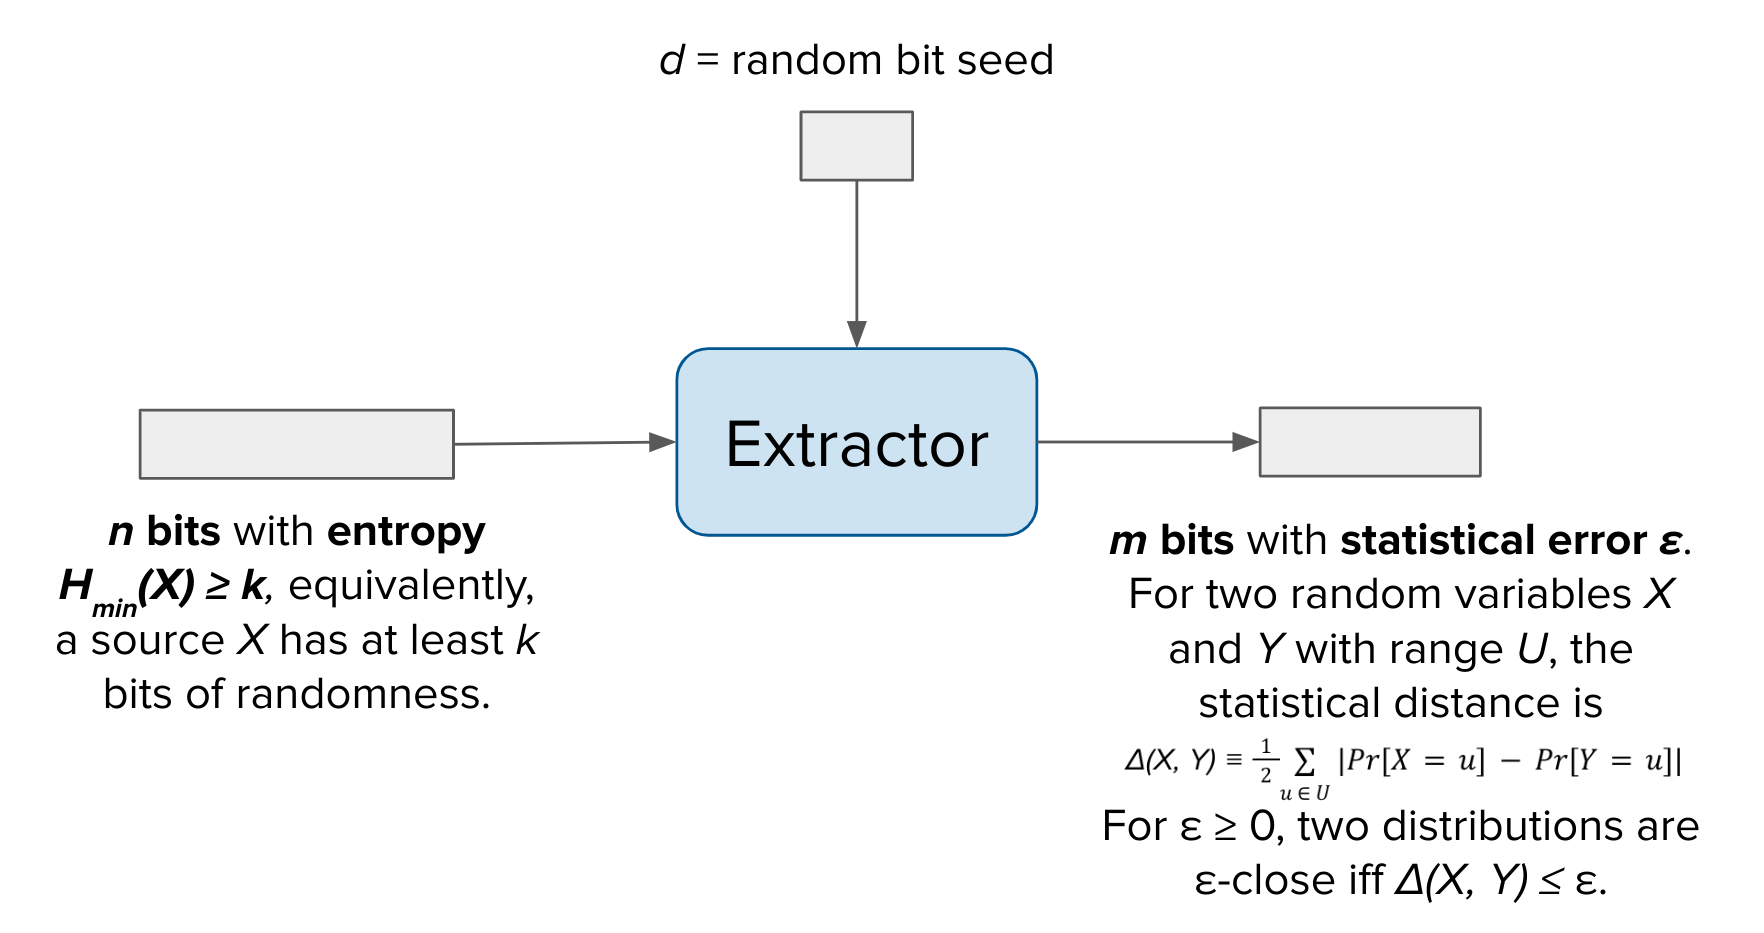
\includegraphics[scale=0.18]{Images/CC_extractor_updated.png}
    \caption{Classical-to-classical (seeded) randomness extractor}
    \label{fig:ExtractorDiagram}
\end{figure}

Recall that our motivation for extractors was to simulate randomization given only a weak random source, or without a seed. If the seed is of logarithmic length, i.e. $d=O(\log n)$, then instead of selecting it randomly we can enumerate all possibilities for the seed and take a majority vote. In summary, the randomness used for seeds can be eliminated by running all the possible seeds and taking the majority value. This is formally defined by the following lemma. 

\begin{lemma}
    Let $A(w,r)$ be a randomized algorithm such that $A(w,U_m)$ has error probability at most $\gamma$, and let $\ibeext:\{0,1\}^n \times \{0,1\}^d \rightarrow \{0,1\}^m$ be a $(k,\varepsilon)$ extractor. Define $A' = {\rm majority}_{y \in \{0,1\}^d} \{A(w, \ibeext(x,y))\}$. Then for every $k$-source\footnote{A random variable $X$ is $k$-source if $H_{\min}(X) \geq k$.} $X$ on $\{0, 1\}^n$, $A'(x, X)$ has error probability of at most $2(\gamma + \varepsilon)$.
\end{lemma}

As stated above, we wish to extract randomness from weak random source $X$ without any additional uniform randomness. Therefore it follows that we want to keep $Y$ as small as possible, even though $X$, and $k$, could be very large. In other words, we would like a long output (i.e. large $m$) using a short seed (i.e. small $d$). This motivates the following definition of strong extractors. 
% The advantage of strong extractors is that the output is close to the uniform distribution even if the value of $U_d$ is known.

\begin{definition}\normalfont{\textbf{(Strong Extractor)}}
    Extractor $\ibeext : \{0, 1\}^n \times \{0, 1\}^d \rightarrow \{0,1\}^m$ is a strong $(k, \varepsilon)$-extractor if for every $k$-source $X$ on $\{0,1\}^n$, $(U_d, \ibeext(X,U_d)$ is $\varepsilon$-close to $(U_d, U_m)$. Equivalently, $\ibeext'(x,y) = (y, \ibeext(x,y))$ is a standard ($k, \varepsilon$)-extractor.
\end{definition}

Before we discuss the explicit construction of a strong extractor, we revisit the question of why the min-entropy is a correct measure to quantify the amount of randomness that can be extracted from a given source? Informally, we can argue that the min-entropy is an upper bound on the amount of randomness that can be extracted: there does not exist any strong extractor that has an output length more than $H_{\min}(X)$. To understand this, first recall that $H_{\min}(X) = - \log P_{\text{guess}}(X)$. Suppose that we now apply some function $f$ to source $X$, then how difficult is it to guess $f(X)$, i.e., what is $P_{\text{guess}}(f(X))?$. Clearly, we can guess $f(X)$ by first guessing $X$ and then applying $f$ to our guess. Thus, we get $P_{\text{guess}}(f(X))\geq P_{\text{guess}}(X)$. However, this is equivalent to
\[H_{\min}(f(X))\leq H_{\min}(X).\]
In other words, this also means that the output of the extractor $\ibeext$ is obtained as a function
$f(X) = \ibeext(X,y)$, for a fixed seed $y$, must have min-entropy at most $H_{\min}(X)$. Thus, the output $\ibeext(X,y)$ can be uniform on at most $H_{\min}(X)$ bits.
How about a converse: does there exist a strong extractor that can extract approximately $H_{\min}(X)$ bits from any $k$-source X? The answer to this question is yes.

We now explore a construction of randomness extractors that achieves well-performing parameters for this application, the 2-universal extractor. Our goal for our parameters is large $m$, or extracting as much randomness as possible, using the smallest possible seed and error, or small $d$ and $\varepsilon$. First, we must define a 2-universal family.
\begin{definition}\normalfont{\textbf{(2-universal family)}}
    A family of hash functions $\mathcal{F} = \{f:\{0,1\}^n \rightarrow \{0,1\}^m\}$ is called \textit{2-universal} if for every two strings $x,x' \in \{0,1\}^n$ with $x \neq x'$, and any two $z, z' \in \{0,1\}^m$, we have
    \[
        \Pr_{f \in \mathcal{F}}[f(x) = z \oplus f(x') = z'] = \frac{1}{2^{2m}}.
    \]
\end{definition}

Using 2-universal families, we are able to define 2-universal extractors as follows.
\begin{definition}\normalfont{\textbf{(2-universal extractor)}}
    Let $\mathcal{F} = \{f_y:\{0,1\}^n \rightarrow \{0,1\}^m, y \in \{0,1\}^d\}$ be a 2-universal family of hash functions such that $|\mathcal{F}| = 2^d$. The associated 2-universal extractor is 
    \[
        \ibeext_{\mathcal{F}}:\{0,1\}^n \times \{0,1\}^d \rightarrow \{0,1\}^m, \ibeext_{\mathcal{F}}(x,y) = f_y(x).
    \]
\end{definition}
Conceptually, consider $\ibeext_{\mathcal{F}}$ as using a seed $y$ to select a function from the family $\mathcal{F}$ uniformly at random and returning the output of the function when evaluated on the source $X$. To evaluate how good this extractor is, we use the leftover hash lemma (insert reference), which is defined as follows.
\begin{definition}\normalfont{\textbf{(Leftover hash lemma)}}
    Let $n$ and $k \leq n$ be arbitrary integers, $\varepsilon > 0$, $m = k - 2\log(\frac{1}{\varepsilon})$, and $\mathcal{F} = \{f: \{0,1\}^n \rightarrow \{0,1\}^m\}$ a 2-universal family of hash functions. Then the 2-universal extractor $\ibeext_{\mathcal{F}}$ is a $(k,\varepsilon)$-strong seeded randomness extractor.
\end{definition}
Due to page limit restrictions, for the leftover hash lemma proof, we refer the reader to \cite{tudelftQC}.

%%% Hey Kyle, Samin wrote the discussion. Could you go through it and check if it looks good?
